\section{Pianificazione}
Nella pianificazione, il \Responsabile{} suddivide il lavoro in attività e le assegna a ciascun membro del gruppo.
Lo scopo è dimostrare come deve essere svolto il lavoro, valutare i progressi nel progetto e anticipare i problemi che potrebbero sorgere preparando delle soluzioni per essi.\\
La pianificazione di progetto viene organizzata seguendo le scadenze presentate nella sezione §1.6.
Lo sviluppo del progetto viene suddiviso nelle seguenti quattro \glo{fasi}: 
\begin{itemize}
	\item Analisi;
	\item Progettazione Architetturale;
	\item Progettazione di Dettaglio e Codifica;
	\item Validazione e Collaudo.
\end{itemize}
Alla fine di ciascuna di queste fasi corrisponde una \glo{milestone} e il gruppo può disporre di una o più \glo{baseline}, base su cui continuare il lavoro nelle successive fasi.\\
Essendo queste fasi di durata di uno o due mesi circa, il gruppo ha ritenuto necessario fare un'ulteriore suddivisione. Ad ogni \glo{fase} corrispondono quindi periodi più brevi, all'interno dei quali vengono elencate le diverse attività che il gruppo \Gruppo{} deve svolgere e gli incrementi previsti.
Alla fine di ciascun periodo corrisponde una \glo{milestone} interna. A differenza delle \glo{milestone} relative alle \glo{fasi}, le cui date vengono stabilite dal calendario del committente, le \glo{milestone} interne sono scelte dal \Responsabile{} del gruppo \Gruppo{}.

\subsection{Analisi}
Periodo: dal 2019-11-15 al 2020-01-20\\
Inizia con la formazione del gruppo e finisce con la data di consegna per la Revisione dei Requisiti.\\
In questa fase viene definito il gruppo, la normazione (\glo{way of working}) e la garanzia di qualità che si vuole fornire, oltre alla definizione dei requisiti del capitolato che viene scelto.

\subsubsection{Periodo 1}
Dal 2019-11-15 al 2019-11-29\\
In questo periodo, che parte dalla formazione del gruppo e termina con la scelta del capitolato C5 \NomeProgetto{}, il gruppo intende affrontare le seguenti tematiche al fine di porre le basi per il lavoro che va affrontato:
\begin{itemize}
	\item \textbf{Discussione capitolati}: Ogni membro del gruppo studia individualmente e in seguito discute con gli altri membri durante gli incontri tutti i capitolati proposti, ponendo le basi per la stesura del documento \SdF{} e indirizzando la scelta del capitolato;
	\item \textbf{Assegnazione e studio dei ruoli di progetto}: Ad ogni membro del gruppo viene assegnato il ruolo principale da ricoprire nella fase di Analisi;
	\item \textbf{Definizione degli strumenti}: Vengono discusse e definite le tecnologie da usare per affrontare la fase di Analisi;
	\item \textbf{Pianificazione milestone fase di Analisi}: Vengono discusse e fissate delle \glo{milestone} intermedie da rispettare per completare la fase di Analisi entro le scadenze imposteci.
\end{itemize}

\subsubsection{Periodo 2} 
Dal 2019-11-30 al 2019-12-31\\
Questo periodo inizia con la scelta definitiva del capitolato C5 \NomeProgetto{}.\\
Dopo la scelta, vanno focalizzate le risorse del gruppo nei seguenti punti:
\begin{itemize}
	\item \textbf{Normazione}: Vengono definite le regole per la stesura dei documenti e per l'utilizzo delle tecnologie identificate in precedenza;
	\item \textbf{Approfondimento capitolati}: Vengono ulteriormente discussi tutti i capitolati in modo da terminare lo \SdF{} e focalizzare l'attenzione sull'analisi del capitolato scelto in modo da predisporre le basi per l'\AdR{};
	\item \textbf{Prima definizione dei casi d'uso}: Attività dove vengono identificati ed analizzati i requisiti del capitolato, cercando di comprendere come il sistema debba essere realizzato;
	\item \textbf{Determinazione standard di qualità}: Vengono definite le strategie per garantire la qualità di \glo{processo} e la qualità di prodotto;
	\item \textbf{Verifica}: \glo{Verifica} dell'andamento del gruppo in relazione alle tempistiche e allo svolgimento dei compiti assegnati.
\end{itemize}

\subsubsection{Periodo 3}
Dal 2020-01-01 al 2020-01-14\\
Questo periodo si estende fino alla data ultima di consegna per affrontare la Revisione dei Requisiti a cui il gruppo ha deciso di partecipare.
\begin{itemize}
	\item \textbf{Normazione}: Ulteriori approfondimenti alle regole per la stesura dei documenti e per l'utilizzo delle tecnologie;
	\item \textbf{Approfondimento delle tecnologie}: Vengono ampliate le conoscenze sulle tecnologie richieste dal capitolato per essere svolto;
	\item \textbf{\AdR{}}: Studio dei requisiti e raffinamento dei casi d'uso;
	\item \textbf{Pianificazione delle attività}: Pianificazione del lavoro da svolgere nelle fasi successive a quella di Analisi;
	\item \textbf{Verifica}: \glo{Verifica} dell'andamento del gruppo in relazione alle tempistiche e allo svolgimento dei compiti assegnati.
\end{itemize}

\subsubsection{Periodo 4} 
Dal 2020-01-15 al 2020-01-20\\
In questo periodo, che ha inizio con la consegna della documentazione prodotta per la Revisione dei Requisiti alla presentazione pubblica della proposta, il gruppo consolida il lavoro svolto in vista delle successive fasi e della discussione per la quale serve una presentazione:
\begin{itemize}
	\item \textbf{Consolidamento}: Ogni membro del gruppo si prende del tempo per ripassare tutto il lavoro svolto e per studiare il necessario per affrontare al meglio le fasi successive;
	\item \textbf{Preparazione per la Revisione dei Requisiti}: Il gruppo produce il materiale necessario da esporre alla presentazione pubblica della propria proposta.
\end{itemize}

%PAGINA ORIZZONTALE
\newpage
\paperwidth=\pdfpageheight
\paperheight=\pdfpagewidth
\pdfpageheight=\paperheight
\pdfpagewidth=\paperwidth
\headwidth=\textheight

\begingroup 
\vsize=\textwidth
\hsize=\textheight

\subsubsection{Diagramma di Gantt delle attività della fase di Analisi}
\pagestyle{empty}
\begin{figure}[h]
	\centering	
	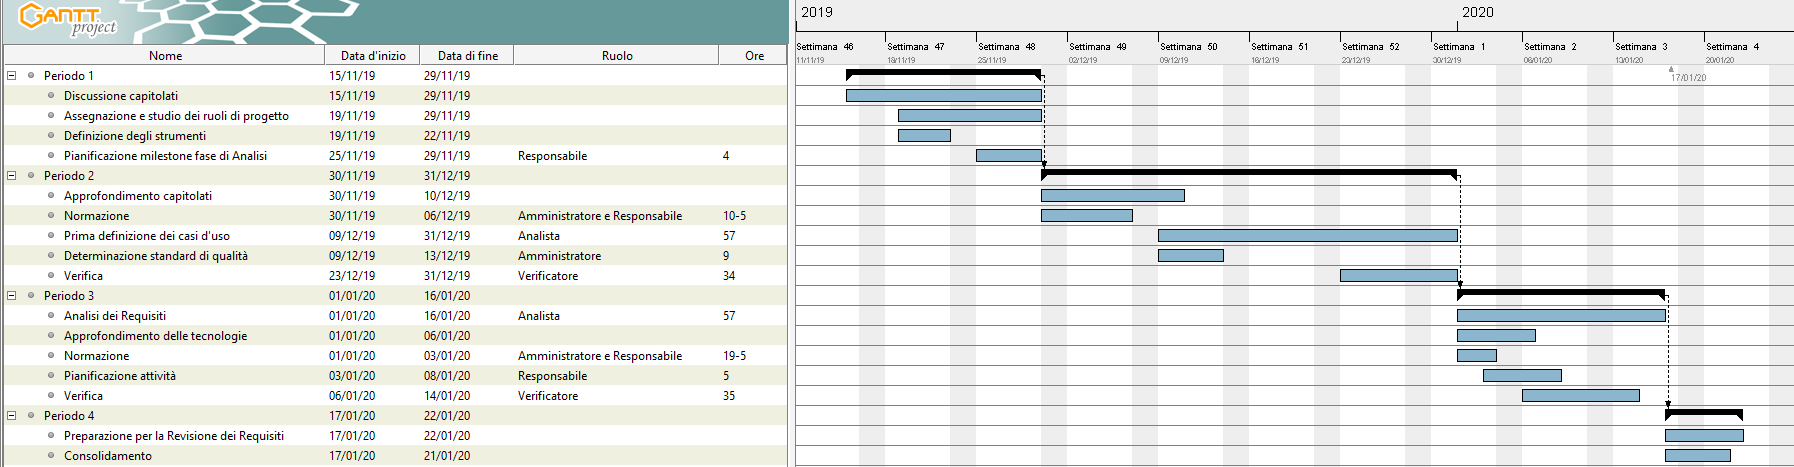
\includegraphics[scale=0.40]{Sezioni/DiagrammiGantt/Analisi.png}
	\caption{Diagramma di Gantt delle attività della fase di Analisi}
\end{figure}

\textwidth=\hsize
\textheight=\vsize

\endgroup
\newpage
\paperwidth=\pdfpageheight
\paperheight=\pdfpagewidth
\pdfpageheight=\paperheight
\pdfpagewidth=\paperwidth
\headwidth=\textwidth

\subsection{Progettazione Architetturale}
Periodo: dal 2020-01-22 al 2020-03-15\\
Inizia al termine della \glo{fase} di Analisi e finisce con la data di consegna per la Revisione di Progettazione.\\
In questa \glo{fase} viene definita una soluzione architetturale in modo da soddisfare i requisiti individuati nella \glo{fase} di Analisi.

\subsubsection{Periodo 1} 
Dal 2020-01-22 al 2020-02-20
\begin{itemize}
	\item \textbf{Normazione}: Standardizzazione e correzione di alcune parti della documentazione che non aderiscono completamente alle \NdP{};
	\item \textbf{\AdR{}}: Avvio della correzione e modifica dei casi d'uso segnalati, concentrandosi sui casi d'uso e requisiti segnalati (e non) utili al \glo{PoC};
	\item \textbf{Assegnazione dei ruoli di progetto}: Assegnazione dei ruoli di ciascun membro del gruppo in base alla suddivisione oraria indicata in §5.2.1;
	\item \textbf{Pianificazione delle attività}: Le attività da svolgere devono essere prima pianificate e discusse dal gruppo per garantire il \glo{way of working} sancito nelle \NdP{};
	\item \textbf{Approfondimento e studio delle tecnologie}: Ricerca di documentazione e materiali utili per l'apprendimento delle nuove tecnologie da utilizzare per la realizzazione del prodotto finale.
	In particolare:
	\begin{itemize}
		\item per l'app per gli utenti: Java per Android, l'\glo{IDE} Android Studio, le \glo{API} di Google per Google Maps, Firebase, Google Play, il formato \glo{JSON}, la libreria client HTTP Volley;
		\item per la web app per gli amministratori: il tool di build automation \glo{Node.js}, i framework \glo{Angular} e \glo{Bootstrap}, \glo{TypeScript};
		\item per il server: il tool di build automation Maven e i suoi \glo{plugin}, gli strumenti di \glo{Swagger} e lo standard \glo{OpenAPI}, il framework Spring per Java, il database \glo{Redis}.
	\end{itemize}
	\item \textbf{Verifica}: \glo{Verifica} dell'andamento del team in relazione alle tempistiche e allo svolgimento dei compiti assegnati.
\end{itemize}

\subsubsection{Periodo 2} 
Dal 2020-02-21 al 2020-03-02
\begin{itemize}
	\item \textbf{Approfondimento delle tecnologie}: \glo{LDAP}, \glo{GPS} per l'app per gli utenti, \glo{Angular} e \glo{Bootstrap} per la web-app per gli amministratori, Spring, \glo{Swagger} e \glo{Redis} per il server;
	\item \textbf{Normazione}: Decisioni ed inserimento delle nuove regole da adottare per le attività di progettazione e sviluppo;
	\item \textbf{Incrementi}: Nella sezione §3.3 sono stati elencati i requisiti sotto forma di incrementi che seguiti in successione portano al prodotto che soddisfa le richieste degli stakeholder.
	In questo periodo viene portato avanti un incremento detto "\textit{Incremento 0}" che ha lo scopo, una volta completato, di fornire una base per il prodotto che deve essere realizzato, facendo comprendere al proponente e al committente
	il modo in cui il gruppo sta lavorando e al gruppo se il proprio \glo{way of working} è buono o va migliorato per poter realizzare con efficacia anche i punti più critici del prodotto richiesto;
	\item \textbf{Progettazione}: Ricerca di una soluzione soddisfacente per tutti gli \glo{stakeholder}, che descriva l'architettura del prodotto prima di pensare al codice, seguendo gli incrementi definiti.
	La definizione dell'architettura deve essere proposta al proponente per ricevere feedback sulla sua bontà;
	\item \textbf{Technology Baseline}: Base per la realizzazione del \glo{Proof of Concept} nell'immediato e della \glo{Product Baseline} successivamente, che dimostra le tecnologie (librerie, framework, linguaggi) selezionati per lo sviluppo del prodotto;
	\item \textbf{Proof of Concept}: Creazione di uno più eseguibili che permettano di dimostrare la validità del prodotto che si vuole fornire, concretizzando la \glo{Technology Baseline}.
	Il \glo{Proof of Concept} realizzato è composto di:
	\begin{itemize}
		\item un'app per utenti sviluppata per dispositivi Android, che fornisca le funzionalità di autenticazione e logout, scaricamento della lista delle organizzazioni, verifica di presenza o meno all'interno dell'\glo{organizzazione} e visionare lo storico degli accessi;
		\item una web app per amministratori che fornisca le funzionalità di autenticazione e logout, scaricamento della lista delle organizzazioni, visualizzazione delle informazioni di un'\glo{organizzazione}, controllo del numero di utenti presenti all'interno dell'\glo{organizzazione};
		\item un server che permetta all'app e alla web-app di ottenere i dati per fornire a utenti e amministratori rispettivamente le funzionalità richieste.
	\end{itemize}
	\item \textbf{Codifica}: Viene codificato il \glo{Proof of Concept} e successivamente condiviso tramite i \glo{repository} del gruppo al committente e al proponente per il colloquio TB in data 3 marzo;
	\item \textbf{Verifica}: \glo{Verifica} dell'andamento del gruppo in relazione alle tempistiche e allo svolgimento dei compiti assegnati.
\end{itemize}

\subsubsection{Periodo 3} 
Dal 2020-03-03 al 2020-03-08
\begin{itemize}
	\item \textbf{Miglioramento standard di qualità}: Aggiunta, rimozione o modifica di alcune metriche per garantire le qualità di \glo{processo} e di prodotto affermate nel \PdQ{};
	\item \textbf{\AdR{}}: Continuazione della correzione del documento alla luce della correzione e del colloquio con il committente in data 2020-02-18;
	\item \textbf{Pianificazione attività}: Aggiustamento delle previsioni precedentemente realizzate sulla base dell'esperienza maturata, in particolar modo dopo la realizzazione del \glo{PoC};
\end{itemize}

\subsubsection{Periodo 4} 
Dal 2020-03-09 al 2020-03-15
\begin{itemize}
	\item \textbf{Consolidamento}: Ogni membro si prende del tempo per ripassare tutto il lavoro svolto e per studiare il necessario per affrontare al meglio le \glo{fasi} successive;
	\item \textbf{Avvio allo studio delle tecnologie mancanti}: Prima dell'avvio della successiva \glo{fase}, cominciare lo studio delle tecnologie non impiegate per il \glo{Proof of Concept} ma necessarie per il prodotto;
	\item \textbf{Preparazione per la Revisione di Progettazione}: Il gruppo produce il materiale necessario da esporre alla presentazione pubblica della propria proposta.
\end{itemize}

%PAGINA ORIZZONTALE
\newpage
\paperwidth=\pdfpageheight
\paperheight=\pdfpagewidth
\pdfpageheight=\paperheight
\pdfpagewidth=\paperwidth
\headwidth=\textheight

\begingroup 
\vsize=\textwidth
\hsize=\textheight

\subsubsection{Diagramma di Gantt delle attività della fase di Progettazione Architetturale}
\pagestyle{empty}
\begin{figure}[h]
	\centering
	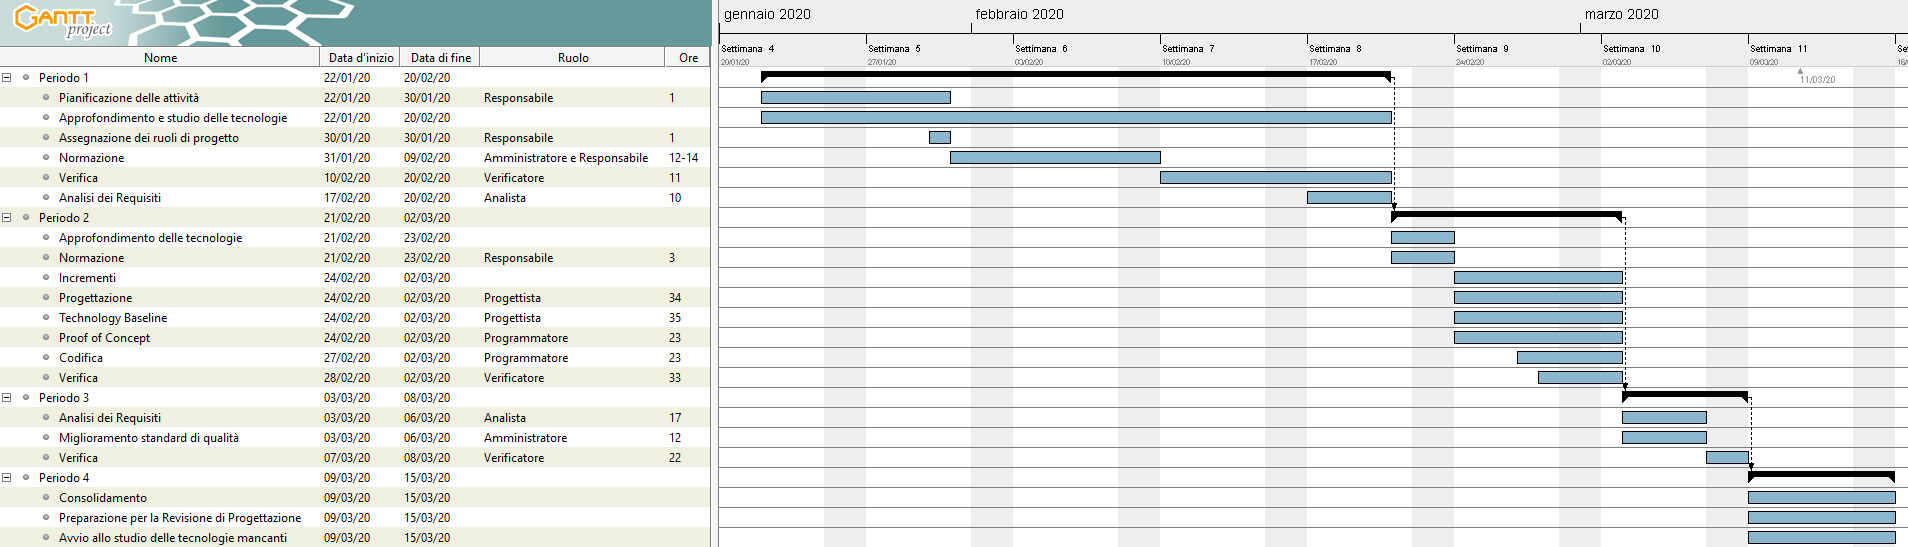
\includegraphics[scale=0.38]{Sezioni/DiagrammiGantt/ProgettazioneArchitetturale.png}
	\caption{Diagramma di Gantt delle attività della fase di Progettazione Architetturale}	
\end{figure}

\textwidth=\hsize
\textheight=\vsize

\endgroup
\newpage
\paperwidth=\pdfpageheight
\paperheight=\pdfpagewidth
\pdfpageheight=\paperheight
\pdfpagewidth=\paperwidth
\headwidth=\textwidth

\subsection{Progettazione di Dettaglio e Codifica}
Dal 2020-03-16 al 2020-05-18\\
Inizia al termine della fase di Progettazione Architetturale e finisce con la data di consegna della Revisione di Qualifica.\\
In questa fase si definisce nel dettaglio e si implementa l'architettura logica costruita nella fase di Progettazione Architetturale.

\subsubsection{Periodo 1} 
Dal 2020-03-16 al 2020-04-07
\begin{itemize}
	\item \textbf{Approfondimento delle tecnologie}: Ricerca documentazione e materiali utili per l'apprendimento delle nuove tecnologie da utilizzare per la realizzazione del prodotto finale;
	\item \textbf{Normazione}: Standardizzazione e correzione di alcune parti della documentazione e che non aderiscono completamente alle \NdP{};
	\item \textbf{Assegnazione dei ruoli di progetto}: Assegnazione dei ruoli di ciascun membro del gruppo in base alla suddivisione oraria indicata in §5.3.1;
	\item \textbf{Pianificazione delle attività}: Le attività da svolgere devono essere prima pianificate e discusse dal gruppo per garantire il \glo{way of working} sancito nelle \NdP{}.
\end{itemize}
\paragraph{Milestone sull'ITS di GitHub}
\begin{itemize}
	\item \href{https://github.com/qb-team/Stalker-Documentazione/milestone/11}{Documentazione};
	\item \href{https://github.com/qb-team/Stalker-App/milestone/1}{App};
	\item \href{https://github.com/qb-team/Stalker-Backend/milestone/1}{Backend};
	\item \href{https://github.com/qb-team/Stalker-Admin/milestone/1}{Admin}.
\end{itemize}

\subsubsection{Periodo 2} 
Dal 2020-04-08 al 2020-05-11
\begin{itemize}
	\item \textbf{Progettazione}: Gli incrementi obbligatori definiti nella sezione §3.3 vengono analizzati e vengono prodotti i diagrammi delle classi, dei package e le relazioni di dipendenza fra essi non ancora analizzati nell'Incremento 0;
	\item \textbf{Implementazione della Product Baseline}: Seguendo le specifiche della \glo{Technology Baseline}, viene realizzata una prima versione stabile del prodotto, \glo{baseline} per il lavoro futuro;
	\item \textbf{Progettazione e codifica incrementale}: Seguendo gli incrementi definiti in §3.3 e la pianificazione temporale in §4.5, i requisiti da soddisfare vengono progettati e successivamente codificati. Per ogni incremento, vengono realizzati:
	\begin{itemize}
		\item diagrammi delle classi;
		\item diagrammi dei package.
	\end{itemize}
	Vengono realizzati inoltre alcuni diagrammi di sequenza per l'app utenti, la web-app amministratori e per il backend, su funzionalità ritenute di rilievo per il sistema da realizzare. In caso di ulteriore tempo a disposizione, vengono realizzati anche dei diagrammi di attività.
	La loro realizzazione viene svolta seguendo lo standard \glo{UML} ed è necessaria per la progettazione delle \glo{REST API}, che seguono invece lo standard \glo{OpenAPI}.
	Una volta che la progettazione di dettaglio di tutto ciò che permette di soddisfare i requisiti degli incrementi è stata completata, si può procedere alla codifica delle tre parti del prodotto software da realizzare: app, web-app, server.
	L'obiettivo del gruppo in questa fase è progettare almeno gli incrementi con i requisiti obbligatori per poter soddisfare gli \glo{stakeholder};
	\item \textbf{Verifica}: \glo{Verifiche} per assicurarsi della bontà dei requisiti implementati;
	\item \textbf{Manuali}: Stesura di almeno una prima versione del Manuale Utente e del Manuale Manutentore in relazione alle funzionalità di base del sistema secondo le regole indicate in \NdP{}.
\end{itemize}
\paragraph{Milestone sull'ITS di GitHub}
\begin{itemize}
	\item \href{https://github.com/qb-team/Stalker-Documentazione/milestone/12}{Documentazione};
	\item \href{https://github.com/qb-team/Stalker-App/milestone/2}{App};
	\item \href{https://github.com/qb-team/Stalker-Backend/milestone/2}{Backend};
	\item \href{https://github.com/qb-team/Stalker-Admin/milestone/2}{Admin}.
\end{itemize}

\subsubsection{Periodo 3}
Dal 2020-05-11 al 2020-05-18
\begin{itemize}
	\item \textbf{Primo rilascio del prodotto}: Pubblicazione del prodotto eseguibile all'interno dei \glo{repository} del gruppo;
	\item \textbf{Verifica}: \glo{Verifica} dell'andamento del team in relazione alle tempistiche e allo svolgimento dei compiti assegnati.
	\item \textbf{Consolidamento}: Ogni membro si prende del tempo per ripassare tutto il lavoro svolto e per studiare il necessario per affrontare al meglio la successiva e ultima fase;
	\item \textbf{Preparazione per la Revisione di Qualifica}: Il gruppo produce il materiale necessario da esporre alla presentazione pubblica della propria proposta.
\end{itemize}
\paragraph{Milestone sull'ITS di GitHub}
\begin{itemize}
	\item \href{https://github.com/qb-team/Stalker-Documentazione/milestone/13}{Documentazione};
	\item \href{https://github.com/qb-team/Stalker-App/milestone/3}{App};
	\item \href{https://github.com/qb-team/Stalker-Backend/milestone/3}{Backend};
	\item \href{https://github.com/qb-team/Stalker-Admin/milestone/3}{Admin}.
\end{itemize}

%PAGINA ORIZZONTALE
\newpage
\paperwidth=\pdfpageheight
\paperheight=\pdfpagewidth
\pdfpageheight=\paperheight
\pdfpagewidth=\paperwidth
\headwidth=\textheight

\begingroup 
\vsize=\textwidth
\hsize=\textheight

\subsubsection{Diagramma di Gantt delle attività di Progettazione di Dettaglio e Codifica}
\pagestyle{empty}
\begin{figure}[h]
	\centering
	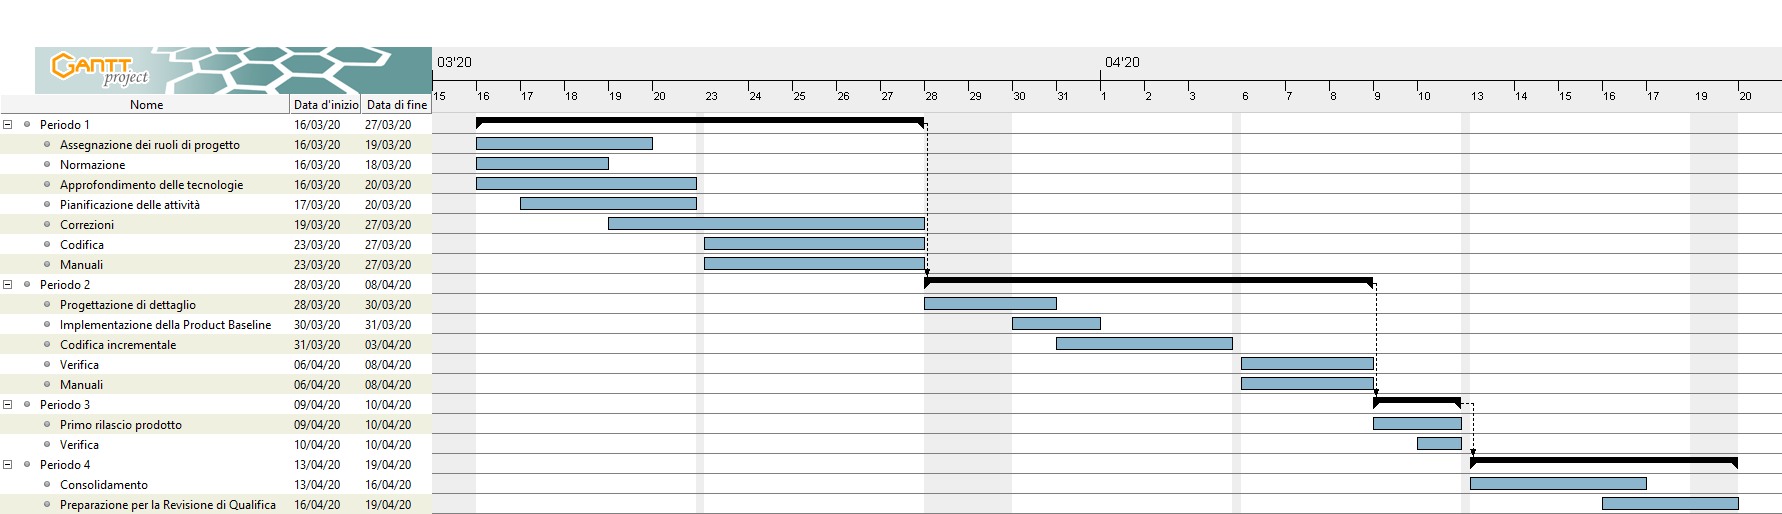
\includegraphics[height = 8cm, width = 24.5cm]{Sezioni/DiagrammiGantt/ProgettazioneDiDettaglio.png}
	\caption{Diagramma di Gantt delle attività di Progettazione di Dettaglio e Codifica}
\end{figure}

\textwidth=\hsize
\textheight=\vsize

\endgroup
\newpage
\paperwidth=\pdfpageheight
\paperheight=\pdfpagewidth
\pdfpageheight=\paperheight
\pdfpagewidth=\paperwidth
\headwidth=\textwidth

\subsection{Validazione e Collaudo}
Dal 2020-04-21 al 2020-05-17\\
Inizia al termine della fase di Progettazione di Dettaglio e Codifica e finisce con la data di consegna per la Revisione di Accettazione.\\
In questo fase vengono definite le attività che servono a verificare che il prodotto corrisponda a quello desiderato dal committente e dal proponente.

\subsubsection{Periodo 1} 
Dal 2020-04-21 al 2020-04-28
\begin{itemize}
	\item \textbf{Normazione}: Standardizzazione e correzione di alcune parti della documentazione che non aderiscono completamente alle \NdP{};
	\item \textbf{Correzioni}: Correzioni di difetti notati dal committente (ove presenti) nella \glo{Product Baseline};
	\item \textbf{Assegnazione dei ruoli di progetto}: Assegnazione dei ruoli di ciascun membro del gruppo in base alla suddivisione oraria indicata in §5.4.1;
	\item \textbf{Soddisfazione dei requisiti}: Controllo che i requisiti siano soddisfatti;
	\item \textbf{Pianificazione attività}: Le attività da svolgere devono essere prima pianificate e discusse dal gruppo per garantire il \glo{way of working} sancito nelle \NdP{};
	\item \textbf{Verifica}: \glo{Verifica} dell'andamento del gruppo in relazione alle tempistiche e allo svolgimento dei compiti assegnati.
\end{itemize}
\paragraph{Milestone sull'ITS di GitHub}
\begin{itemize}
	\item \href{https://github.com/qb-team/Stalker-Documentazione/milestone/15}{Documentazione}
\end{itemize}

\subsubsection{Periodo 2} 
Dal 2020-04-29 al 2020-05-10
\begin{itemize}
	\item \textbf{Codifica}: Esecuzione dell'ultimo versionamento del prodotto;
	\item \textbf{Verifica}: Accertamento che le esecuzioni delle attività siano esenti da errori (condizione necessaria ma non sufficiente: superamento dei test di unità, di integrazione, di sistema);
	\item \textbf{Validazione}: Verifica se il prodotto realizzato sia conforme alle attese, e validazione finale in caso di esito positivo;
	\item \textbf{Scrittura dei manuali}: Esecuzione del secondo versionamento del Manuale Utente e del Manuale Manutentore;
	\item \textbf{Collaudo}: Vengono eseguiti gli ultimi test sul prodotto per verificare se le funzionalità rispettano i risultati attesi.
\end{itemize}
\paragraph{Milestone sull'ITS di GitHub}
\begin{itemize}
	\item \href{https://github.com/qb-team/Stalker-Documentazione/milestone/16}{Documentazione}
\end{itemize}

\subsubsection{Periodo 3} 
Dal 2020-05-11 al 2020-05-17
\begin{itemize}
	\item \textbf{Preparazione per la Revisione di Accettazione}: Il gruppo produce il materiale necessario da esporre alla presentazione pubblica della propria proposta.
\end{itemize}
\paragraph{Milestone sull'ITS di GitHub}
\begin{itemize}
	\item \href{https://github.com/qb-team/Stalker-Documentazione/milestone/17}{Documentazione}
\end{itemize}

%PAGINA ORIZZONTALE
\newpage
\paperwidth=\pdfpageheight
\paperheight=\pdfpagewidth
\pdfpageheight=\paperheight
\pdfpagewidth=\paperwidth
\headwidth=\textheight

\begingroup 
\vsize=\textwidth
\hsize=\textheight

\subsubsection{Diagramma di Gantt delle attività di Validazione e Collaudo}
\pagestyle{empty}
\begin{figure}[h]
	\centering
	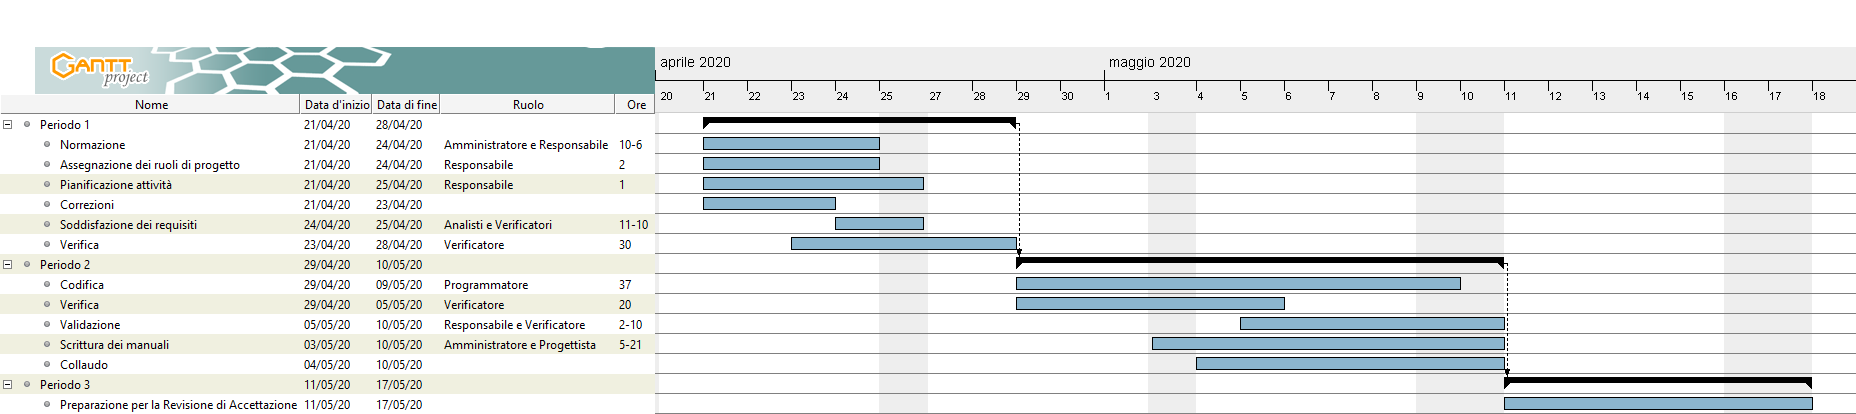
\includegraphics[scale=0.40]{Sezioni/DiagrammiGantt/Validazione.png}
	\caption{Diagramma di Gantt delle attività di Validazione e Collaudo}
\end{figure}

\textwidth=\hsize
\textheight=\vsize

\endgroup
\newpage
\paperwidth=\pdfpageheight
\paperheight=\pdfpagewidth
\pdfpageheight=\paperheight
\pdfpagewidth=\paperwidth
\headwidth=\textwidth

%PAGINA ORIZZONTALE
\newpage
\paperwidth=\pdfpageheight
\paperheight=\pdfpagewidth
\pdfpageheight=\paperheight
\pdfpagewidth=\paperwidth
\headwidth=\textheight

\begingroup 
\vsize=\textwidth
\hsize=\textheight

\subsection{Pianificazione temporale degli incrementi}
\pagestyle{empty}
\begin{figure}[h]
	\centering
	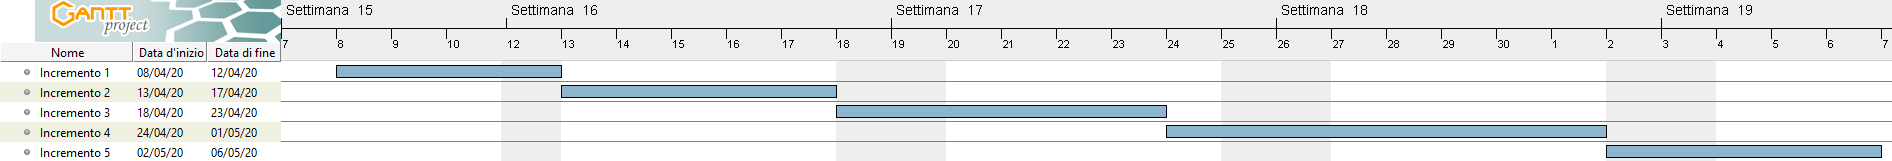
\includegraphics[height = 4cm, width = 24.5cm]{Sezioni/DiagrammiGantt/PianificazioneTemporaleIncrementi.png}
	\caption{Diagramma di Gantt degli incrementi del Periodo 2 della Fase di Progettazione di Dettaglio e Codifica}
\end{figure}

\begin{figure}[h]
	\centering
	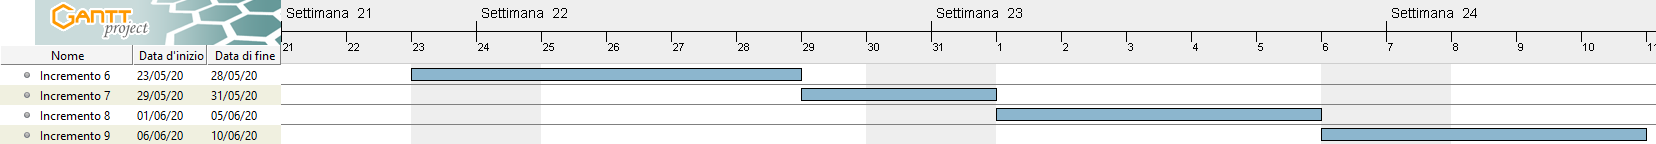
\includegraphics[height = 4cm, width = 24.5cm]{Sezioni/DiagrammiGantt/PianificazioneTemporaleIncrementi2.png}
	\caption{Diagramma di Gantt degli incrementi del Periodo 2 della Fase di Validazione e Collaudo}
\end{figure}

\textwidth=\hsize
\textheight=\vsize

\endgroup
\newpage
\paperwidth=\pdfpageheight
\paperheight=\pdfpagewidth
\pdfpageheight=\paperheight
\pdfpagewidth=\paperwidth
\headwidth=\textwidth